\documentclass[class=article, crop=false, 12pt]{standalone}
\usepackage[subpreambles=true]{standalone}
\usepackage{../.common/common}


\author{Tony Shing}
%\pretitle{Supplementary}

\topic{Note 6C (Mechanics)}
\title{Central Force Motion}

\version{2025} % leave blank for omitting

\begin{document}

\maketitle

%\heading{Lecture}{Tony}

\begin{overview}
    \begin{itemize}
        \item Equation of motion for central force motion, and its standard solution.
        \item Deriving Kelper's Laws. 
        \item Equation of motion for two-bodies system - reducible to one-body motion.
    \end{itemize}
\end{overview}


% content begins here
% Section %%%%%%%%%%%%%%%%%%%%%%%%%%%%%%%%%%%%%%%%%%%%%%%%%%%%
\section{The General Solution}

An object undergoes a central force motion if it is moving in a potential that depends purely on the radial coordinate of the object. 
i.e. $V(r,\theta, \phi) = V(r)$. The Newton's \nth{2} law simply writes:
\aleq{
    \Aboxed{
        m\dv[2]{\vvec{r}}{t} = -\dv{V(r)}{r}
    }
}


\red{Such potential is guarenteed to be conservative}, 
by showing that the curl on the force is $0$.

\begin{notation}[]
    \ul{The steps to show curl = 0} (Out of syllabus) :

    \begin{enumerate}
        \item The force only has radial component and also solely depends on the radial coordinate.
        \aleq{
            \vvec{F}(r,\theta, \phi) &= -\grad V(r) \\[1ex]
            %
            &\defeq -\gradSph{V(r)} \\[1ex]
            %
            &= -\pdv{V(r)}{r}\hhat{r} + 0 + 0 \\
            &= f(r)\hhat{r}
        }
        %
        \item Then apply curl in spherical coordinate. 
        Observe that all the terms vanish by knowing that 
        $F_\theta = F_\phi = 0$ and $F_r$ is a function on $r$ only.
        \aleq{
            \curl \vvec{F} &\defeq \curlSph{F_r}[F_\theta][F_\phi] \\[1ex]
            &= \text{ (all terms = 0) }
        }
    \end{enumerate} 
\end{notation}


%%%%%%%%%%%%
\subsection{Standard Derivation} 

(\it{Every textbook does the same proof})

\begin{itemize}
    \item The force from potential is the only force and is conservative $\Rightarrow$ Energy conserves.
    \aleq{
        E = \half m\norm{\hhat{v}}^2 + V(r) = \half m \qty[\qty(\dv{r}{t})^2+\qty(r\dv{\theta}{t})^2] + V(r)= \text{const}
    }
    \item Force is along radial direction $\Rightarrow$ Torque = 0 $\Rightarrow$ Angular momentum conserves.
    \aleq{
        L = m \vvec{r}\cross\vvec{v} = m r^2 \dv{\theta}{t} = \text{const}
    }
\end{itemize}

The standard rundown is to treat $E$ and $L$ as adjustable parameters 
and derive the function of the object's trajectory $r(\theta)$.

\label{standard proof}
\begin{enumerate}
    \item Substitute the equation of $L$ into equation of $E$ and rearange terms.
    \aleq{
        E &= \half m \qty[\qty(\dv{r}{t})^2+\qty(\frac{L}{mr})^2] +V(r)\\[0.5em]
        \Rightarrow\ \dv{r}{t} &= \sqrt{\frac{2}{m}\qty(E-V(r) - \frac{L^2}{2mr^2})}
    }
    \item By $L = mr^2 \dv{\theta}{t} \Rightarrow \dd{t} = \frac{mr^2}{L}\dd{\theta}$, then move all terms that contain $r$ to one side.
    \aleq{
        \dv{r}{t} = \frac{L}{mr^2}\dv{r}{\theta} 
        &= \sqrt{\frac{2}{m}\qty(E-V(r) - \frac{L^2}{2mr^2})} \\[0.5em]
        %
        \dd{\theta} 
        &= \cub[blue]{\inv{r^2}\frac{1}{\sqrt{\frac{2mE}{L^2} - \frac{2mV(r)}{L^2} - \inv{r^2}}}}
            {\substack{\text{This is}\\\text{a function of }r\text{ only.}}}\dd{r}
    }
    This expression is ready to be integrated, 
    but first we need to specify $V(r)$.
\end{enumerate}


%%%%%%%%%%%%
\subsection{Power Law Potential}

A function satisfies \bf{power law} if it is in the form $f(x)\sim x^\alpha$ for any real number $\alpha$. 
Most of the time we deal with potential function belongs in such form, 
i.e. $V(r) = kr^\alpha$. The most common ones are:
\begin{itemize}
    \item $\alpha=-1$ : Columb's Law / Newtonian gravity -- $V(r) = \pm \frac{k}{r}$
    \item $\alpha=2$ : Simple harmonic motion -- $V(r) = \half k r^2$
\end{itemize}

Substituting the power law potential, 
mathematicians found that the integral can be resolved into simple functions only when $\alpha = 2, -1$ or $-2$.  




\linesep
% Section %%%%%%%%%%%%%%%%%%%%%%%%%%%%%%%%%%%%%%%%%%%%%%%%%%%%
\section{Case $\alpha=-1$: Inverse square force}

The R.H.S integral is ready to be integrated. 
First substitute $u=\dinv{r}$ and $\dd{u}=-\dinv{r^2}\dd{r}$.
Then simplify by trigonometric substitution. 
\aleq{
    \int\dd{\theta} &= \int\inv{r^2}\frac{\dd{r}}{\sqrt{\frac{2mE}{L^2} - \frac{2mV(r)}{L^2} - \inv{r^2}}}\\
    %
    &= -\int\frac{\dd{u}}{\sqrt{\frac{2mE}{L^2} - \frac{2mV(u^{-1})}{L^2} - u^2}}
    & {\scriptstyle \qty(\text{subst. }u=\inv{r},\, \dd{u}=-\inv{r^2}\dd{r})}\\
    %
    &= -\int\frac{\dd{u}}{\sqrt{\frac{2mE}{L^2} \red{\pm} \frac{2m\red{ku}}{L^2} - u^2}} \\
    %
    &= -\int\frac{\dd{u}}{\sqrt{\frac{2mE}{L^2} + \frac{m^2k^2}{L^4} - \qty(u \mp \frac{mk}{L^2})^2}} 
    & \qty(\substack{\text{completing}\\\text{square}}) \\
    %
    &= -\int \frac{\dd{\qty(u\mp\frac{mk}{L^2})}}{\sqrt{A^2 - \qty(u\mp\frac{mk}{L^2})^2}}
    & {\scriptstyle \qty(\text{take }A = \sqrt{\frac{2mE}{L^2} + \frac{m^2k^2}{L^4}})} \\
    %
    &= -\int \frac{\dd\qty(A\cos{\phi})}{\sqrt{A^2-A^2\cos^2\phi}}
    & {\scriptstyle \qty(\text{take } u\mp\frac{mk}{L^2} = A\cos{\phi})} \\
    %
    &= \int \dd{\phi} \\
    %
    &= \cos^{-1}\qty(\frac{u\mp\frac{mk}{L^2}}{\sqrt{\frac{2mE}{L^2} + \frac{m^2k^2}{L^4}}}) + C\\
    %
    \theta &= \cos^{-1}\qty(\frac{\frac{L^2}{mk\red{r}}\mp 1}{\sqrt{\frac{2EL^2}{mk^2} + 1}}) + C 
    & {\scriptstyle \qty(\text{subst. }u=\inv{r} \text{ and rearrange terms})} \\
    %
    \Aboxed{\inv{r} &= \frac{mk}{L^2}\qty(\sqrt{1+\frac{2EL^2}{mk^2}}\cos{\qty(\theta -C)} \pm 1)}
}
where the $\pm$ sign is for: \red{$+$ve = attractive force, $-$ve = repulsive force.} 
This formula is usually written in a less complicated form by using these symbols:
\begin{itemize}
    \item $\boxed{\epsilon \defeq \sqrt{1+\frac{2EL^2}{mk^2}}}  =$ \bf{encentricity}
    
    \item $\theta_0 \defeq C =$ some initial angle
    
    \item $\dinv{r_0} \defeq \dfrac{mk}{L^2}  =$ reciprocol to some initial radial distance
    
\end{itemize} 

And becomes the \bf{polar equation} of trajectory.
\aleq{
    \inv{r} &= \inv{r_0}\qty(\epsilon\cos{\qty(\theta-\theta_0)}\pm 1) \\
    \Aboxed{
        r &= \frac{r_0}{\epsilon\cos{\qty(\theta -\theta_0)} \pm 1}
        \qquad \qty(\substack{\text{+ve for attractive}\\\text{-ve for repulsive}})
    }
}


%%%%%%%%%%%%%%%%%
\subsection{Kepler's \nth{1} Law - Equation of Trajectory}

The original statement from Kepler only concerns elliptical/circular orbits in gravitation, 
because they were the only types of orbits observed.

\quoting{The orbit of every planet is an ellipse with the sun at one of the two foci.}

With coordinate geometry, we can show that \red{every conic sections are possible trajectories}. 
Convert to cartesian coordinate by substituting $r=\sqrt{x^2+y^2}$, $\cos{\theta}=\frac{x}{r}$ 
and $\sin{\theta}=\frac{y}{r}$,
\aleq{
    r &= \frac{r_0}{\epsilon\cos{\qty(\theta -\theta_0)} \pm 1}\\[0.8ex]
    %
    \pm r &= r_0 - r\epsilon\cos{(\theta-\theta_0)}\\[0.8ex]
    %
    r^2 &= r^2\epsilon^2\cos^2{(\theta-\theta_0)} - 2rr_0\epsilon\cos{(\theta-\theta_0)} + r_0^2 \\[0.8ex]
    %
    &= r^2\epsilon^2\qty[\cos\theta\cos\theta_0 + \sin\theta\sin\theta_0]^2 
        - 2rr_0\epsilon \qty[\cos\theta\cos\theta_0 + \sin\theta\sin\theta_0] + r_0^2\\[0.8ex]
    %
    x^2 + y^2 &= \epsilon^2\qty[x\cos\theta_0 + y\sin\theta_0]^2 
        - 2r_0\epsilon \qty[x\cos\theta_0 + y\sin\theta_0] + r_0^2\\[0.8ex]
    %
    \Aboxed{
    \qty(\epsilon^2\cos^2\theta_0-1)x^2 + &\qty(\epsilon^2 \sin^2\theta_0-1)y^2 
        + \qty(2\epsilon^2\sin{\theta_0}\cos{\theta_0})xy 
        -(2\epsilon r_0\cos\theta_0) x - (2\epsilon r_0 \sin\theta_0) y + r_0^2 = 0
    }
} 

we arrive at the \bf{quadratic form} of conic sections, 
i.e. $Ax^2+Bxy+Cy^2+Dx+Ey+F=0$, 
regardness of the force being central attractive or repulsive.
Usually textbooks begin their analysis by choosing $\theta_0 = 0$, 
essentially making the conic section "lies flat".
\aleq{
    (\epsilon^2-1)x^2 - y^2 - (2\epsilon r_0)x + r_0^2 &= 0\\[0.8ex]
    %
    x^2 - \frac{2\epsilon}{\epsilon^2-1}x - \frac{y^2}{\epsilon^2-1} &= -\frac{r_0^2}{\epsilon^2-1}
    & \qty({\scriptstyle\text{Divide }\epsilon^2-1})\\[0.8ex]
    %
    \qty(x + \frac{r_0\epsilon }{1-\epsilon^2})^2 - \frac{r_0^2\epsilon^2}{(1-\epsilon^2)^2} 
        + \frac{y^2}{1-\epsilon^2} &= \frac{r_0^2}{1-\epsilon^2} 
        & \qty({\scriptstyle\text{Completing squares}})\\[0.8ex]
    %
    \qty(x + \frac{r_0\epsilon }{1-\epsilon^2})^2 + \frac{y^2}{1-\epsilon^2} 
        &= \qty(\frac{r_0}{1-\epsilon^2})^2 \\[0.8ex]
    %
    \frac{\qty(x + \frac{r_0\epsilon}{1-\epsilon^2})^2}{\qty(\frac{r_0}{1-\epsilon^2})^2} 
        + \frac{y^2}{\qty(\frac{r_0}{\sqrt{1-\epsilon^2}})^2} &= 1 \\[0.8ex]
    %
    \Rightarrow \quad 
    \Aboxed{
        \frac{(x+c)^2}{a^2} + \frac{y^2}{b^2} &= 1
    }
} 

This is the \bf{standard form}, another common way to present conic section.\\

Conventionally, no matter what kinds of conic section it is, 
we identify these letters with the following names.
Although they are mostly used in circular/elliptical orbits because they are positive real number only if $\epsilon<1$.

\begin{itemize}
    \item \bf{Semi-latus rectum} \,--\, $\cbox[red]{r_0 \defeq \frac{L^2}{mk}}$ \qquad (also commonly denoted by $l$ in books)
    \item \bf{Semi-major axis} \,--\, $\cbox[red]{a \defeq \frac{r_0}{1-\epsilon^2} = -\frac{k}{2E}}$
    \item \bf{Semi-minor axis} \,--\, $\boxed{b \defeq \frac{r_0}{\sqrt{1-\epsilon^2}}}$ 
    \item \bf{Focal distance} \,--\, $\boxed{c \defeq \frac{r_0\epsilon}{1-\epsilon^2} = a\epsilon}$ 
        \qquad\qquad  (Another name for $c$ = linear encentricity)
\end{itemize}

\red{\bf{\ul{Note:}} The definition of $a$ and $r_0$ are the most important to remember,
because we can compute the object's energy and angular momentum directly from them.}
\aleq{
    \Acboxed[red]{
        \bcase{
            E &= -\dfrac{k}{2a}\\[1ex]
            L &= \sqrt{mkr_0}
        }
        \qquad \text{(True for all orbits)}
    }
}

(You can also re-derive the definition of encentricity from them).\\

The value of $\epsilon$ determines the ratio of $a,b,c$ relative to $r_0$, 
so as the type of conic section. 

\begin{center}
    \begin{minipage}{0.8\linewidth}
        \centering
        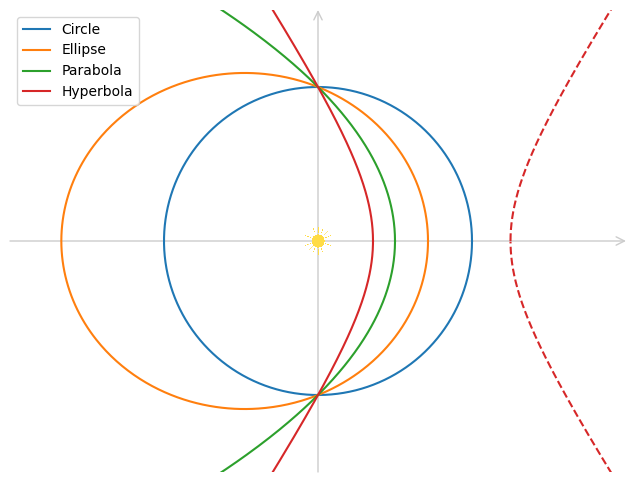
\includegraphics[width=\textwidth]{all_traj}
    \end{minipage}
\end{center}


\newpage
%%%%%%%%%%%%%%
\subsubsection{$\epsilon = 0$ \,--\, Circle}

\begin{itemize}
       
    \item \ul{Standard form}: We can see that $a=b=r_0$ and $c=0$. 
    \aleq{
        \Aboxed{
            x^2 + y^2 =r_0^2
        }
    }
    which is the equation of a circle at center $(0,0)$ and radius $r_0$.

    \item \ul{Polar equation}: $r=\dfrac{r_0}{\epsilon\cos\theta \pm 1} = \dfrac{r_0}{0 \pm 1} = \pm r_0$. 
    \begin{itemize}
        \item Attractive force ($+$ve) : Radial distance = $r_0$ = constant.
        \item Repulsive force ($-$ve) : $r<0$ is not physical. 
        i.e. Trajectory cannot be a circle if the central force is repulsive.
    \end{itemize}
    
    \item \ul{Energy}: By substituting $\epsilon=0$ to $a$, $\boxed{E=-\frac{k}{2r_0}}$.
\end{itemize}
\begin{center}
    \begin{minipage}{0.8\linewidth}
        \centering
        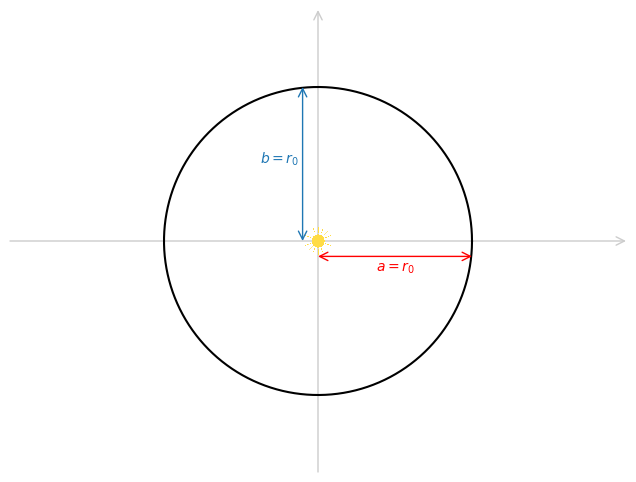
\includegraphics[width=\textwidth]{circle}
    \end{minipage}
\end{center}

\newpage
%%%%%%%%%%%%%%
\subsubsection{$0<\epsilon <1$ \,--\, Ellipse}

\begin{itemize}
    \item \ul{Standard form}: We have $a= \dfrac{r_0}{1-\epsilon^2} > \dfrac{r_0}{\sqrt{1-\epsilon^2}} = b$.
    \aleq{
        \Aboxed{
            \frac{(x+a\epsilon)^2}{a^2} + \frac{y^2}{b^2} = 1
        }
    }
    This is the equation of an ellipse with its center shifted to $(-a\epsilon,0)$,
    while $(0,0)$ becomes one of the foci of the ellipse.

    \item \ul{Polar equation}:
    
    \begin{itemize}
        \item Attractive force ($+$ve) : $r=\dfrac{r_0}{\epsilon\cos\theta + 1}$,
        which is in the range between:
        \begin{itemize}
            \item The \bf{perihelion} point - When $\theta=0$, $r$ is min - $\boxed{r_p = \frac{r_0}{1+\epsilon}}$
            
            \item The \bf{aphelion} point - When $\theta=\pi$, $r$ is max - $\boxed{r_a = \frac{r_0}{1-\epsilon}}$
        \end{itemize}
    
        \item Repulsive force ($-$ve) : $r=\dfrac{r_0}{\epsilon\cos\theta - 1} <0$ is not physical. 
        i.e. Trajectory cannot be an ellipse if the central force is repulsive.

    \end{itemize}
    
    \item \ul{Energy}: By substituting $\epsilon$ and $r_0$ into $a$, $\boxed{ -\dfrac{mk^2}{2L^2} < E < 0}$
\end{itemize}

\begin{center}
    \begin{minipage}{0.8\linewidth}
        \centering
        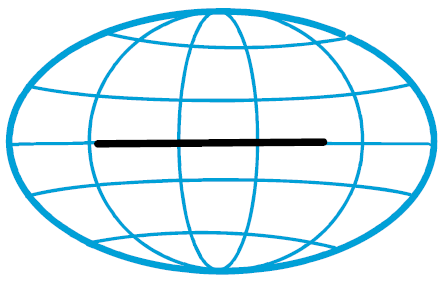
\includegraphics[width=\textwidth]{ellipse}
    \end{minipage}
\end{center}


%%%%%%%%%%%%%%
\subsubsection{$\epsilon=1$ \,--\, Parabola}

\begin{itemize}
    

    \item \ul{Standard form}: $a,b,c$ all becomes infinite. 
    So the standard form becomes meaningless. 
    In fact, we have to re-derive it from the first step:
    \aleq{
        \ccancelto[green]{0}{(\epsilon^2-1)}x^2 - y^2 - (2\ccancelto[green]{1}{\epsilon} r_0)x + r_0^2 &= 0 \\
        \Aboxed{
            -\inv{2r_0}y^2 + \frac{r_0}{2} &= x
        }
    }
    This a quadratic equation, i.e. parabola, but lying horizontally. 
    The tip is at $\qty(\dfrac{r_0}{2},0)$.

    \item \ul{Polar form}:
    \begin{itemize}
        \item Attractive force ($+$ve) : $r=\dfrac{r_0}{\cos\theta + 1}$,
        which is in the range between:
        \begin{itemize}
            \item The \bf{perihelion} point - When $\theta=0$, $r$ is min - $\boxed{r_p = \frac{r_0}{2}}$
            
            \item The \bf{aphelion} point does not exist - When $\theta=\pi$, $r=\infty$.
        \end{itemize}
    
        \item Repulsive force ($-$ve) : $r=\dfrac{r_0}{\cos\theta - 1} <0$ is not physical. 
        i.e. Trajectory cannot be a parabola if the central force is repulsive.

    \end{itemize}

    \item \ul{Energy}: By substituting $\epsilon=1$ to the encentricity's definition, $\boxed{E=0}$


\end{itemize}

\begin{center}
    \begin{minipage}{0.8\linewidth}
        \centering
        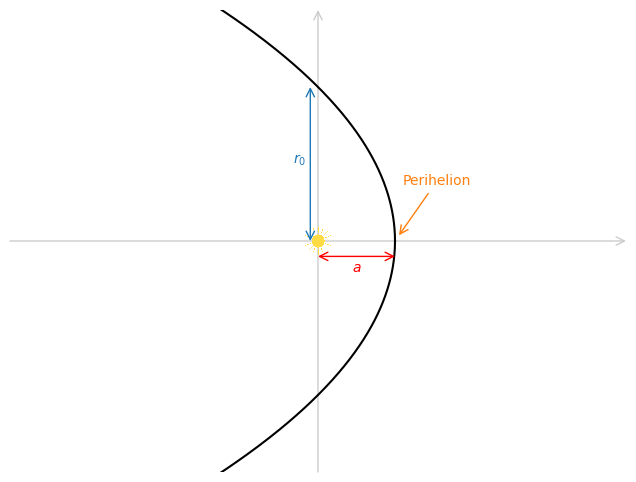
\includegraphics[width=\textwidth]{parabola}
    \end{minipage}
\end{center}


%%%%%%%%%%%%%%
\subsubsection{$\epsilon>1$ \,--\, Hyperbola}

\begin{itemize}
    \item \ul{Standard form}: $a,c < 0$ and $b$ becomes imaginary. 
    Take out the magnitude part: $b=i\cdot \dfrac{r_0}{\sqrt{\epsilon^2-1}} = ib'$,
    the standard form becomes:
    \aleq{
        \Aboxed{
            \frac{(x+a\epsilon)^2}{a^2} - \frac{y^2}{b'^2} &= 1
        }
    }
    This is the equation of an hyperbola with its center shifted to $(-a\epsilon,0)$,
    while $(0,0)$ becomes one of the foci of the ellipse.
    The trajectories on two sides are corresponding to the cases of attractive and repulsive force.

    \item \ul{Polar form}: $r=\dfrac{r_0}{\epsilon\cos\theta \pm 1} > 0$ only if $\cos\theta > \mp\dinv{\epsilon}$.
    \begin{itemize}
        \item Attractive force ($+$ve) : 
        
        \begin{itemize}
            \item The \bf{perihelion} point - When $\theta=0$, $r$ is min - $\boxed{r_p = \frac{r_0}{1+\epsilon}}$
            
            \item The \bf{aphelion} point does not exist - When $\cos\qty(\pm\theta) = -\dinv{\epsilon}$, $r=\infty$.
    
        \end{itemize}

        \item Repulsive force ($-$ve) : 
        \begin{itemize}
            \item The \bf{perihelion} point - When $\theta=0$, $r$ is min - $\boxed{r_p = \frac{r_0}{\epsilon-1}}$
            
            \item The \bf{aphelion} point does not exist - When $\cos\qty(\pm\theta) = \dinv{\epsilon}$, $r=\infty$.
    
        \end{itemize}
    \end{itemize}
        

    \item \ul{Energy}: By substituting $\epsilon$ and $r_0$ into $a$, $\boxed{E > 0}$
    

\end{itemize}

\begin{center}
    \begin{minipage}{0.8\linewidth}
        \centering
        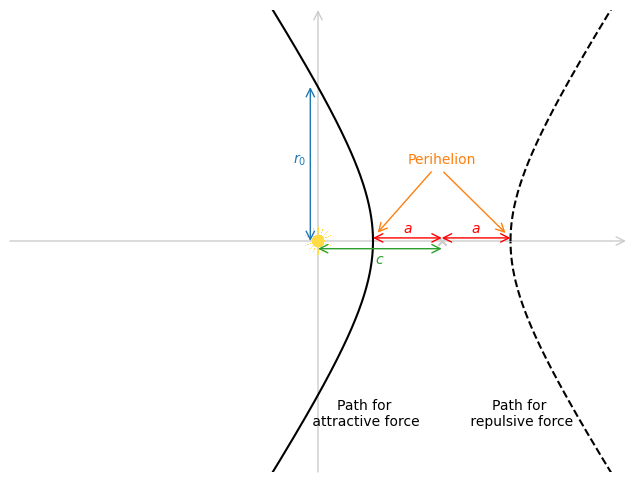
\includegraphics[width=\textwidth]{hyperbola}
    \end{minipage}
\end{center}





%%%%%%%%%%%%%%%%%
\subsection{Kepler's \nth{2} Law - Conservation of Angular Momentum}

The original statement for Kelper's \nth{2} Law says:

\quoting{A line joining a planet and the Sun sweeps out equal areas during equal intervals of time.}

With our physics knowledge nowadays, 
we know that this statement is equivalent to saying "\bf{angular momentum conserves along an orbit}".
The statement is written in this way because the concept of angular momentum did not exist during Kelper's life 
(Newton was birth after Kepler's death).\\

With the equations derived previously, we can show:

\begin{itemize}
    \item The angle $\theta$ of an arc is related to sweeping time by $\dd{t} = \dfrac{mr^2}{L}\dd{\theta}$
    \item The arc's area is $\displaystyle \iint r\dd{\theta}\dd{r} = \int \half r^2 \dd{\theta}$
\end{itemize}

Combining,

\aleq{
    \text{Area}_{(t_2-t_1)} = \int_{t_1}^{t_2} \half \cdot \frac{L}{m} \dd{t} \ \tkn{kepler2}{=}\  \frac{L}{2m}{(t_2-t_1)}
}
\addArrow[red]{kepler2}{(0,4.5ex)}{$\substack{\text{True only if}\\L \text{ is NOT a function of }t}$}
{(0,1.5ex)}{(0,1.5ex)}

Note that this is true even for parabola and hyperbola orbits.

\begin{center}
    \begin{minipage}{0.7\linewidth}
        \centering
        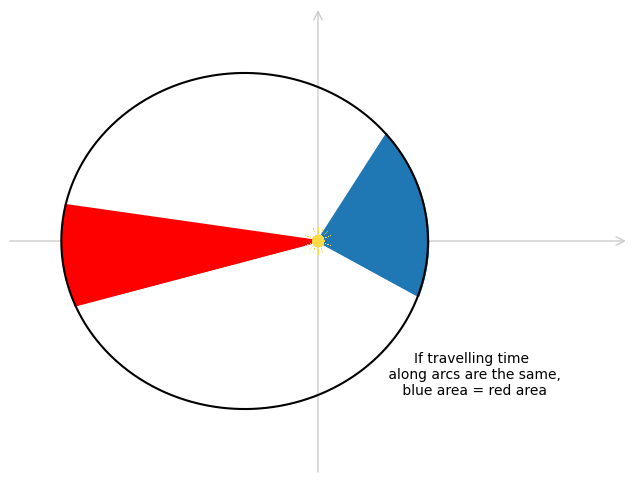
\includegraphics[width=\textwidth]{kelper2}
    \end{minipage}
\end{center}


\newpage
%%%%%%%%%%%%%%%%%
\subsection{Kepler's \nth{3} Law - Period of Elliptical Orbit}

The original statement for Kepler's \nth{3} Law only applies to circular and elliptical orbit, 
because the concept of "period" only applies to closed orbits. 

\begin{center}
    \vskip 1em
    \begin{minipage}{0.9\textwidth}
        \quoting{The ratio of the square of an object's orbital period with the cube of the semi-major axis of its orbit 
            is the same for all objects orbiting the same primary object.}
    \end{minipage}
\end{center}

\vskip 1em
If we go back to the standard proof in section \ref{standard proof} and stop at step 1, 
without substituting $\dd{t} = \frac{mr^2}{L}\dd{\theta}$, 
we can integrate and obtain a relation between $t$ and $r$.

\aleq{
    \dd{t} &= \frac{\dd{r}}{\sqrt{\frac{2}{m}\qty(E-V(r) - \frac{L^2}{2mr^2})}} \\[1ex]
    %
    &= \frac{\dd{r}}{\sqrt{\frac{2}{m}\qty(E \red{\pm\frac{k}{r}} - \frac{L^2}{2mr^2})}} 
    & \qty(\substack{+\ : \text{ attractive} \\-\ : \text{ repulsive}}) \\[0.5em]
    %
    \int \dd{t} &= \sqrt{-\frac{m}{2E}} \int \frac{r\dd{r}}{\sqrt{r^2 \mp \frac{k}{E}r + \frac{L^2}{2mE}}}
    & \qty(\substack{\text{Denominator} \\\text{multiply }-\frac{r^2}{E}}) \\[1ex]
    %
    &= \sqrt{-\frac{m}{2E}} \int \frac{r\dd{r}}{\sqrt{-\qty(r\mp\frac{k}{2E})^2+\frac{k^2}{4E^2}+\frac{L^2}{2mE}}}
    & \qty(\substack{\text{completing}\\\text{square}})
}

Substitute $a=-\frac{k}{2E}$ and $a^2\epsilon^2 = \frac{k^2}{4E^2}\qty(1+\frac{2EL^2}{mk^2})$ to simplify the notations. 
\aleq{
    \Rightarrow \int \dd{t} &= \sqrt{-\frac{m}{2E}} \int \frac{r\dd{r}}{\sqrt{-(r\pm a)^2+a^2\epsilon^2}}\\[1ex]
    %
    &= \sqrt{-\frac{m}{2E}} \int \frac{(a\mp a\epsilon\cos{\varphi}) \dd{(a \mp a\epsilon\cos{\varphi})}}{\sqrt{a^2\epsilon^2-(a\epsilon\cos{\varphi})^2}}
    & {\scriptstyle \qty(\text{take } r = a \,\mp\, a\epsilon\cos{\varphi})} \\[1ex]
    %
    &= \sqrt{-\frac{m}{2E}} \int \frac{(a\mp a\epsilon\cos{\varphi})}{a\epsilon\sin{\varphi}} (\pm a\epsilon\sin{\varphi})\dd{\varphi}\\[1ex]
    %
    &= \sqrt{-\frac{m}{2E}} \int (\pm a - a\epsilon\cos{\varphi}) \dd{\varphi}\\[1ex]
    %
    &= \sqrt{-\frac{m}{2E}} (\pm a-a\epsilon\sin{\varphi} )  + C\\[1ex]
    %
    &= \sqrt{\frac{a}{k}}(\pm a -a\epsilon\sin{\varphi} )  + C
    & {\scriptstyle \qty(\text{by } a = -\frac{k}{2E})}
}

The symbol $\varphi$ is commonly denoted as the \bf{eccentric anomaly}.
Note that the above is derived without removing the $\pm$ sign, 
so the definition applies to both attractive and repulsive force cases.

\newpage
Algebraically, $\varphi$ and $\theta$ can be inter-converted through their relations with $r$. 
Although this can be done only  numerically. 
\aleq{
    \cub[red]{\frac{r_0}{\epsilon\cos{\theta} \pm 1} }{\text{Polar Equation}} 
    \ =\ r\ &=\
    \cub[blue]{ a \mp a\epsilon\cos{\varphi}}{\text{Definition of }\varphi} \\[1ex]
    %
    \Rightarrow \quad \frac{r_0}{a} = 1-\epsilon^2 
    = (\text{A constant}) &= (1\mp \epsilon \cos{\varphi})(1\pm \epsilon\cos{\theta})
}


Then we can immediately check that in elliptical orbit, 
$\theta = 0 \Leftrightarrow \varphi = 0$ and $\theta=\pi \Leftrightarrow \varphi=\pi$. 
So taking $\varphi$ from $0$ to $2\pi$ is the same as revolving one cycle of $\theta$ from $0$ to $2\pi$. 
Substitute these into the $t$ v.s. $\varphi$ relation, we arrive at the familar Kepler's \nth{3} law formula.
\aleq{
    \text{1 Period} = \int^T_0 \dd{t} 
    &= \eval{\sqrt{\frac{a}{k}}(\red{+} a -a\epsilon\sin{\varphi})}_{\varphi =0}^{\varphi =2\pi} \\
    \Aboxed{
        T &= \frac{2\pi}{\sqrt{k}}a^{\frac{3}{2}}
    }
}


\begin{notation}[Side note:]
    In an elliptical orbit, we can view $\varphi$ as a parmetrization to the standard form:
    \aleq{
        \frac{(x+a\epsilon)^2}{a^2} + \frac{y^2}{b^2} = 1
        \qquad\Rightarrow\qquad
        \text{take}\quad \bcase{
            x+a\epsilon &= a\cos{\varphi}\\
            y &= b\sin{\varphi}
        }
    }

    \vskip 1ex
    \begin{center}
        \begin{minipage}{0.48\linewidth}
            \centering
            \red{\ul{x coordinate $= -(a\epsilon - a\cos{\varphi})$}\\}
            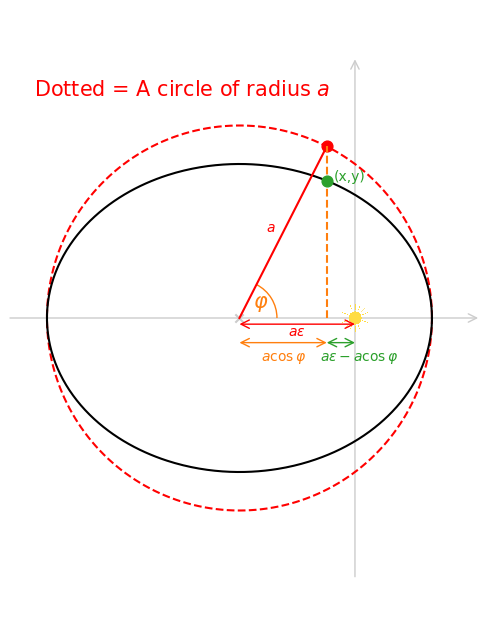
\includegraphics[width=\textwidth, trim=0 80 0 30, clip]{ea1}
        \end{minipage}
        \begin{minipage}{0.48\linewidth}
            \centering
            \blue{\ul{y coordinate $= b\sin{\varphi}$}\\}
            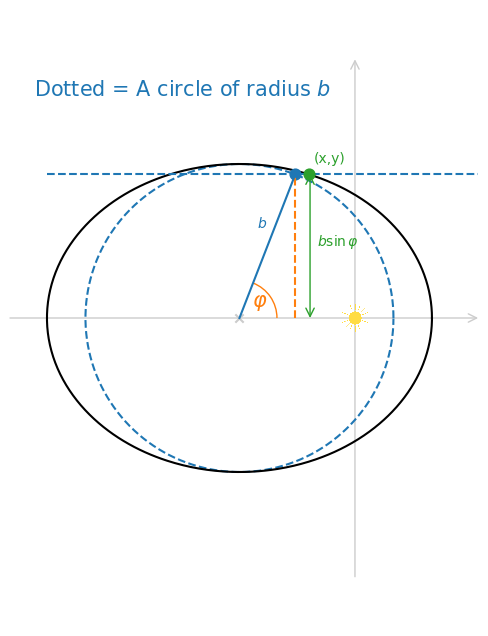
\includegraphics[width=\textwidth, trim=0 80 0 30, clip]{ea2}
        \end{minipage}
    \end{center}

\end{notation}
\begin{notation}[]
    We can verify that the distance from the origin $\sqrt{x^2+y^2}$ is exactly $r=a-a\epsilon\cos{\varphi}$.
    \aleq{
        x^2 + y^2 &= (a\epsilon - a\cos\varphi)^2 + (b\sin\varphi)^2\\
        &= \qty(\frac{r_0}{1-\epsilon^2})^2(\epsilon - \cos\varphi)^2 + \qty(\frac{r_0}{\sqrt{1-\epsilon^2}})^2(\sin\varphi)^2\\
        &= \qty(\frac{r_0}{1-\epsilon^2})^2\qty(\epsilon^2-2\epsilon\cos\varphi + \cos^2\varphi + (1-\epsilon^2)\sin^2\varphi)\\
        &= \qty(\frac{r_0}{1-\epsilon^2})^2\qty(1-2\epsilon\cos\varphi + \epsilon^2\cos^2\varphi)\\[1ex]
        &= a^2(1-\epsilon\cos\varphi)^2
    }

    Moreover, in hyperbola orbit, the parametrization by $\varphi$ becomes
    \aleq{
        \frac{(x+a\epsilon)^2}{a^2} - \frac{y^2}{b^2} = 1
        \qquad\Rightarrow\qquad
        \text{take}\quad \bcase{
            x+a\epsilon &= a\cosh{\varphi}\\
            y &= b\sinh{\varphi}
        }
    }

    Trajectory are more frequently expressed in terms of $\varphi$ in space engineering texts because 
    the $t$ v.s. $\varphi$ relation is readily available for computing transit time.
    \aleq{
        t - t_0 = \sqrt{\frac{a}{k}}(\pm a -a\epsilon\sin{\varphi})
    }

    It is a lot easier than using $\theta$.

\end{notation}



\linesep
% Section %%%%%%%%%%%%%%%%%%%%%%%%%%%%%%%%%%%%%%%%%%%%%%%%%%%%
\section{Two-body Problem Reduction}

In a two body system, where their interaction forces satisfy:
\begin{itemize}
    \item its magnitude that only depends on the distance between the two objects.
    \item its direction is along the line that connects the two objects.
\end{itemize} 
Then it is easy to show that the equation of motions can be rewritten into the form of one body subjecting to the same force. 
Thus we can solve their trajectories by solving only 1 ODE.

\vskip 0.5em
\underline{\textit{Proof}}\par
\hspace{0.025\textwidth}\begin{minipage}{0.95\linewidth}
\vskip 0.5em

    The pairs of Newton \nth{2} Law should start in this form:
    \aleq{
        \begin{cases}
            m_1\dvv[2]{\vvec{r}_1}{t} &= \vvec{F}(\abs{\vvec{r}_2-\vvec{r}_1}) \\[1em]
            m_2\dvv[2]{\vvec{r}_2}{t} &= -\vvec{F}(\abs{\vvec{r}_{2}-\vvec{r}_1})
        \end{cases}
    }

\end{minipage}

\begin{minipage}{0.95\linewidth}
    We can immediately see that, after dividing the masses and subtracting one of them by the other, we arrive at
    \aleq{
        \dv[2]{\vvec{r}_2}{t} - \dvv[2]{\vvec{r}_1}{t} &= -\qty(\inv{m_2}+\inv{m_1})\vvec{F}(\abs{\vvec{r}_{2}-\vvec{r}_1})\\
        \Rightarrow \qquad \dv[2]{\vvec{u}}{t} &= -\qty(\inv{m_2}+\inv{m_1})\vvec{F}(\abs{\vvec{u}}) 
    }

    by taking $\vvec{u} = \vvec{r}_2 - \vvec{r}_1$. It is common to denote $\mu = \inv{\inv{m_1}+\inv{m_2}}$ as the \bf{reduced mass}, 
    so that it is equivalent to the Newton \nth{2} Law describing an object of mass $\mu$ moving along its trajectory $\vvec{u}$ subjecting to a force $-\vvec{F}(\abs{\vvec{u}})$. 
    On the other hand, adding the two equation gives the Newton \nth{2} Law about the center of mass, $\vvec{r}_{CM} = \frac{m_1\vvec{r}_1+m_2\vvec{r}_2}{m_1+m_2}$:
    \aleq{
        m_2\dv[2]{\vvec{r}_2}{t} + m_1\dvv[2]{\vvec{r}_1}{t} &= 0 \\
        \Rightarrow \qquad \dv[2]{t}\qty(m_1\vvec{r}_1+m_2\vvec{r}_2) &= \dv[2]{t}\qty(\frac{m_1\vvec{r}_1+m_2\vvec{r}_2}{m_1+m_2}) = 0
    }


    Now the problem is reduced to two independent ODEs --- a still annoying one for $\vvec{u}$ that involves the central force,
    and a trivial one for $\vvec{r}_{CM}$.
    \aleq{
        \Acboxed{
            \begin{cases}
                \mu\dvv[2]{\vvec{u}}{t} = -\vvec{F}(\abs{\vvec{u}}) \\[1em]
                \dvv[2]{\vvec{r}_{CM}}{t} = 0
            \end{cases}
        }
    }

    which is comparatively easier than solving a system of 2 ODEs. 

    
\hfill $\square$
\end{minipage}
\vskip 1.5em \par

Finally with $\vvec{u}$ and $\vvec{r}_{CM}$, we can retrieve back $\vvec{r}_1$ and $\vvec{r}_2$ by the geometric relation.
\aleq{
    \begin{cases}
        \vvec{r}_1 = \vvec{r}_{CM} - \frac{m_2}{m_1+m_2}\vvec{u} \\
        \vvec{r}_2 = \vvec{r}_{CM} + \frac{m_1}{m_1+m_2}\vvec{u}
    \end{cases}
}



\theend
\end{document}